\documentclass[11pt]{article}
\usepackage{acl2016}
\usepackage{times}
\usepackage{latexsym}
\usepackage{amsmath, amssymb, amsthm, amsfonts}
\usepackage{multirow}
\usepackage[hidelinks]{hyperref}
\usepackage{hyperref}
\usepackage{float}
\usepackage{enumitem}
\setlist{nosep}
\usepackage{subcaption}
\usepackage{soul}
\hypersetup{
    bookmarks=false,         % show bookmarks bar?
    unicode=false,          % non-Latin characters in Acrobat’s bookmarks
    colorlinks=true,       % false: boxed links; true: colored links
    linkcolor=red,          % color of internal links (change box color with linkbordercolor)
    citecolor=black,        % color of links to bibliography
    filecolor=magenta,      % color of file links
    urlcolor=blue           % color of external links
}
\usepackage{tikz}
\usetikzlibrary{arrows,shapes,snakes,automata,backgrounds,petri,positioning}



% To expand the titlebox for more authors, uncomment
% below and set accordingly.
% \addtolength\titlebox{.5in}    

\newcommand{\fix}{\marginpar{FIX}}
\newcommand{\new}{\marginpar{NEW}}
\newcommand{\NIL}{\mbox{\textsc{nil}}}
\newcommand{\qtext}[1]{\texttt{#1}}

\title{Collective Entity Resolution with Multi-Focal Attention}

% Author information can be set in various styles:
% For several authors from the same institution:
% \author{Author 1 \and ... \and Author n \\
%         Address line \\ ... \\ Address line}
% if the names do not fit well on one line use
%         Author 1 \\ {\bf Author 2} \\ ... \\ {\bf Author n} \\
% For authors from different institutions:
% \author{Author 1 \\ Address line \\  ... \\ Address line
%         \And  ... \And
%         Author n \\ Address line \\ ... \\ Address line}
% To start a seperate ``row'' of authors use \AND, as in
% \author{Author 1 \\ Address line \\  ... \\ Address line
%         \AND
%         Author 2 \\ Address line \\ ... \\ Address line \And
%         Author 3 \\ Address line \\ ... \\ Address line}
% If the title and author information does not fit in the area allocated,
% place \setlength\titlebox{<new height>} right after
% at the top, where <new height> can be something larger than 2.25in
\author{Author1 \and Author2\\
	    Google Inc. \\
	    1600 Amphitheatre Pkwy\\
	    Mytown, NY 10000, USA\\
	    {\tt author1@google.com}}

\date{}

\begin{document}
\maketitle

\begin{abstract}
Entity resolution is the task of linking each mention of an entity in
text to the corresponding record in a knowledge base (KB).  Coherence
models for entity resolution encourage all referring expressions in a
document to resolve to entities that are related in the KB. 
We explore attention-like mechanisms for coherence, where the evidence for each
candidate is based on a small set of strong relations, rather than relations
to all other entities in the document. 
The rationale is that document-wide support may simply not exist 
for non-salient entities, or entities not densely connected in the KB.
 Integrating our approach with an existing competitive baseline system improves its
performance on three (out of three) benchmarks, yielding
state-of-the-art results on the TAC KBP 2011 and 2012 tasks.
\end{abstract}

\newcommand{\be}{\begin{equation}}
\newcommand{\ee}{\end{equation}}
\newcommand{\bea}{\begin{eqnarray*}}
\newcommand{\eea}{\end{eqnarray*}}

\renewcommand{\eqref}[1]{Eq.~(\ref{#1})}
\newcommand{\figref}[1]{Fig. \ref{#1}}
\newcommand{\secref}[1]{Sec. \ref{#1}}
\newcommand{\amax}{\text{amax}}
\newcommand{\samax}{\text{samax}}

\newtheorem{theorem}{Theorem}[section]
\newtheorem{lemma}[theorem]{Lemma}
\newtheorem{proposition}[theorem]{Proposition}

\newcommand{\reals}{\field{R}}
\newcommand{\field}[1]{\mathbb{#1}}
\newcommand{\phiv}{\boldsymbol{\phi}}

\newcommand{\fs}{\phiv_s(x,y_i)}
\newcommand{\fp}{\phiv_p(x,y_i,y_j)}
\newcommand{\ww}{\boldsymbol{w}} 
\newcommand{\ws}{\ww_s}
\renewcommand{\wp}{\ww_p}


\section{Introduction}
\label{sec:intro}

Named entity resolution and disambiguation (NERD) is the task of mapping each mention of an entity in a document to the corresponding record in a knowledge base (KB) \cite{BunescuP06,Cucerzan07,KulkarniSRC09,Dredze2010,Hoffart2011,Hachey2013130}.  
 %with numerous applications \cite{Gabrilovich2007,Lin2012,Kwiatkowski2011,finin2009Coreference,mayfield2009cross}. 
%Key applications 
%are to information extraction  and grounded semantic parsing. %text classification~\cite{Gabrilovich2007}, 
%information extraction~\cite{Lin2012} and grounded semantic parsing~\cite{Kwiatkowski2011}. 
%It can also provide a valuable signal to other language-processing tasks, including part-of-speech tagging, parsing, and coreference resolution~\cite{finin2009Coreference,mayfield2009cross}.
%Entity resolution
This is a challenging problem, as referring expressions are often ambiguous on their own, and can only be resolved given appropriate context. For example, the mention \qtext{Beirut} may refer to the capital of Lebanon, to the indie band from New Mexico, or to a drinking game. Names may also refer to entities that are not in the KB, a problem known as \emph{{\NIL} detection}. 
Entity resolution applications include numerous language-processing tasks  \cite{Gabrilovich2007,Lin2012,finin2009Coreference,mayfield2009cross}. \todo{rephrase}%Kwiatkowski2011

Systems for entity resolution typically consist of a \emph{mention model}, a \emph{context model}, and a \emph{coherence model}.\todo{refs} The mention model establishes a link between each entity and its textual representations, also called aliases or surface forms. The context model helps resolve an ambiguous phrase using textual features extracted from the surrounding context, such as the enclosing sentence and salient noun phrases in the document. The coherence model, which is our focus in this work, encourages all mentions to resolve to entities that are related to each. This relation may defined via
the KB, web links or other resources. 

Coherence models are often specified via a graph whose vertices are candidate entities for all mentions, and whose edges express relations between candidate entities for these mentions.\footnote{An exception to this framework are topic models in which a topic may generate both entities and words, e.g. \cite{kataria2011,HanS12,houlsby2014scalable}.}  Vertex weights correspond to prior scores for candidate entities, while edge weights correspond to some notion of relation strength. There exist different ways to leverage such a graph for inference purposes. Broadly speaking, all methods define a score function over whole document disambiguation, and see a labeling that maximizes this score. However, since maximizing the score is typically intractable, various approximations and heuristics are employed.\todo{refs}

Here we propose to enhance coherence models by introducing a multi-focal attention mechanism. Attention has recently been used with considerable empirical success in tasks such as translation \cite{bahdanau2014neural} and image caption generation \cite{xu2015show}. For NERD, we argue that attention is desirable since  aggregating support for an entity label over the whole document may dilute the evidence for non-salient entities. Instead, we propose a model where each mention {\em chooses} a small set of mentions to attend to, and then uses those to calculate its coherence score. 

We show how such an approach can result in a simple inference algorithm, and how the model parameters can be  learned from data. We also
provide a smoothed version of the attention function, that generalizes the soft-max function used in single-focus attention schemes. 

Finally, we evaluate our model by using a context model from the recently introduced Plato system \cite{Lazic2015} (note that Plato does not use a coherence model). This leads to performance improvements on three benchmarks, and yields new state-of-the-art results on the TAC KBP 2010-2012 datasets, and the CoNLL 2003 dataset.\todo{be more specific}

Our contributions thus consist of defining a novel multi-focal attention based model, where inference is efficient, and applying it successfully to an entity linking system. We note that our model can be easily applied to other structured prediction problems in NLP.\todo{Consider expanding this}
%Our premise is that this may also hold for entity relations: aggregating support for an entity label over the whole document may dilute the evidence for non-salient entities. We explore two new approaches to coherence that focus on a \emph{limited number} of relations for each candidate, rather than relations to all other entities. 

\begin{figure*}[!ht]
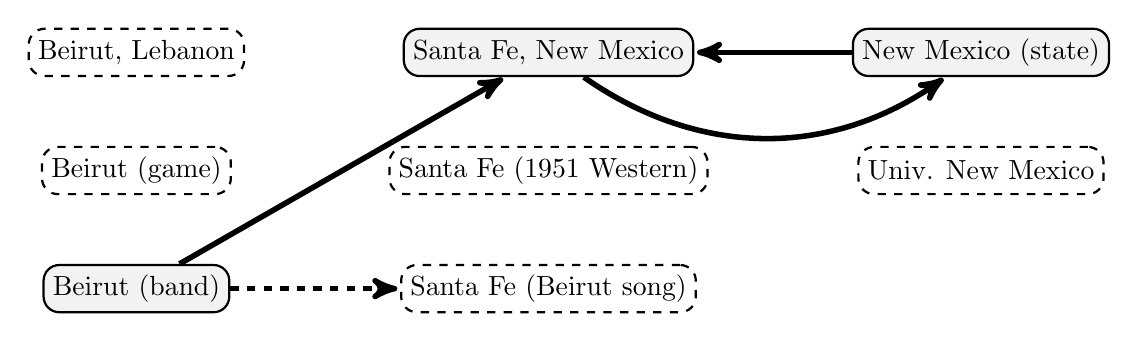
\begin{tikzpicture}[node distance=1.5cm,>=stealth',bend angle=35,auto]
  \tikzstyle{candidate}=[rectangle,dashed,rounded corners=2mm,thick,draw=black,fill=white,minimum size=6mm]
  \tikzstyle{selected} = [rectangle,rounded corners=2mm,thick,draw=black,fill=gray!10,minimum size=6mm]
  \tikzstyle{mention}=[rectangle,thick,draw=black!75,
  			  fill=black!10,minimum size=6mm]
  \tikzstyle{every label}=[black]

 \begin{scope}
    % First mention.
   % \node [mention] (m1){\qtext{Beirut}};
   % \node [candidate] (c11) [label=above:0.5] {Beirut, Lebanon};
   \node [candidate] (c11) {Beirut, Lebanon};
    \node [candidate] (c12) [below of=c11]  {Beirut (game)};
        \node [selected] (c13)  [below of=c12] {Beirut (band)};

   % Second mention.
   % \node [mention] [right=3cm of m1](m2){\qtext{Santa Fe}};
    \node [selected] (c21) [right=2cm of c11] {Santa Fe, New Mexico};
        \node [candidate] (c22) [below of=c21]  {Santa Fe (1951 Western)};
    \node [candidate] (c23)  [below of=c22] {Santa Fe (Beirut song)};

      
     % Third mention.
   % \node [mention] [right=3cm of m2](m3){\qtext{New Mexico}};
    \node [selected] (c31) [right=2cm of c21] {New Mexico (state)};
    \node [candidate] (c32)  [below of=c31] {Univ. New Mexico};
 
      
   %\path (c13) edge [post,line width=2pt] node[above]{0.5} (c21);
   \path (c13) edge [post,line width=2pt] (c21);
   \path (c13) edge [post,dashed,line width=2pt] (c23);
   \path (c31) edge [post,line width=2pt] (c21);
   \path (c21) edge [post,line width=2pt,bend right] (c31);
  \end{scope}
\end{tikzpicture}
\caption{Example coherency graph for mentions $\qtext{Beirut}$, $\qtext{Santa Fe}$ and $\qtext{New Mexico}$. Solid lines indicate a valid solution subgraph, where each selected candidate has at most one outgoing edge to another candidate. TODO: better example?}
\label{fig:graph}
\end{figure*}

%  Accordingly, we propose to choose the label for each mention based on the best support from a \emph{limited number} of other mentions.  In other words,  each mention is labeled by (tractable) inference in a star graph, but one where most edges are (dynamically) ignored.
\comment{
\subsection{Our contributions}
\label{sec:intro:our}


In the first approach, which we name \emph{single link}, we formulate inference as finding the highest-weight subgraph in which each candidate has a directed edge to \emph{at most} one other candidate. This can roughly be seen as maximizing over relations as opposed to averaging. In this model we perform inference using max-sum belief propagation \cite{Kschischang2001}.

%; however, it is slightly more computationally involved since an edge between two entities is allowed only if the corresponding mentions resolve to them. 
%We specify the objective and constraints using binary edge-indicator variables, and find the maximum-a-posteriori solution using the max-sum algorithm \cite{Kschischang2001}. 
Our

In the second \emph{attention} model, we allow each mention to have up to $K$ relations to other mentions. In this case, inference is tractable, and we also learn mention and edge scores from a small set of simple features.   %In other words,  each mention is labeled by (tractable) inference in a star graph, but one where most edges are (dynamically) ignored.

We use these coherence models to re-rank candidates generated by Plato \cite{Lazic2015}, a recent entity resolution system that has highly competitive performance and does not include a coherence component. This leads to performance improvements on three benchmarks, and yields new state-of-the-art results on the TAC KBP 2011 and 2012 datasets.
}
\todo{paper layout}



\section{Definitions and notation}
\label{sec:notation}

We are given a document with $n$ mentions, where each mention $i$ has a set of $n_i$ candidate entities $\mathcal{C}_i = \{c_{i,1}, ..., c_{i,n_i}\}$. The goal is to assign a label $y_i \in \mathcal{C}_i$ to each mention.

Similarly to previous work, our approach to disambiguation relies on local and pairwise candidate scores, which we denote by $s_i(y_i)$ and $s_{ij}(y_i, y_j)$ respectively. The local score is based only on local evidence, such as the mention phrase and textual features, while the pairwise score is based on the relatedness of the two candidates. 
In Sections \ref{sec:score_param} and \ref{sec:learning} we discuss how these scores may be parameterized and learned.  Many systems \cite{Cucerzan07,Milne2008,KulkarniSRC09} simply hardwire pairwise scores.

%In the \emph{single link} model, we compute these scores deterministically and use them as fixed model inputs. In the \emph{attention} model, we parameterize the scores and learn them using a labeled dataset.

Coherence models typically attempt to maximize a {\em global} objective function that assigns a score to each complete labeling ${\bf y} = (y_1,\ldots, y_n)$. 
%, given the local and pairwise scores. 
An example of such a function is the sum of all singleton and pairwise scores for each label:\footnote{The scores usually depend not only on the labels, 
but also on the input text. We omit this dependence for brevity.}
 %A common example of such a function $g(y_1,\ldots,y_n)$ is:
\be
g({\bf y}) = \sum_i s_i(y_i) + \sum_i \sum_{j :  j \neq i} s_{ij}(y_i,y_j).
\label{eq:global_obj}
\ee 
One disadvantage of this approach is that maximizing $g$ corresponds to finding the MAP assignment of a general pairwise Markov random field, and is hence
NP hard for the general case \cite{wainwright2008graphical}. Another limitation is that non-salient entities may be related to very few other entities mentioned in the document, and summing over all mentions may dilute the evidence for such entities. In this paper we explore alternative objectives, relying on attention and tractable inference.



%%% Local Variables: ***
%%% mode:latex ***
%%% TeX-master: "main.tex"  ***
%%% tex-main-file: "main.tex"  ***
%%% End: ***

\section{Model Definition}
Assume we have $n$ mentions we wish to disambiguate. The $i^{th}$ mention will have $n_i$ candidates and we denote those by $c_1,\ldots, c_{n_i}$. The goal 
of the entity linking model is to assign a label $y_i\in \{c_1,\ldots, c_{n_i}\}$ to each mention.

As with other coherence based approaches, we use local and pairwise scorews. Local scores are denoted by $s_i(y_i)$, and score each candidate $y_i$ for the $i^{th}$ mention based on local evidence (e.g., context, mention text etc). The pairwise scores are denoted by $s_{i,j}(y_i,y_j)$ and score each candidate pair based on its coherence. 

In what follows, we first describe the inference part of our model. Namely, how to predict the labels $y_i$ given the scores. We later explain how scores are claculated and learned.

\section{Single-link model}
\label{sec:maxsum}

To motivate our modeling choices of using multi-focal attention and decomposed inference, we additionally consider a simple baseline model with single-focus attention and global inference. In this approach, which we name \emph{single link}, each mention $i$ attends to exactly one other mention that maximizes the pairwise relation score. The corresponding objective can be written as
\begin{align}
g^{SL}({\bf y}) &= \sum_i \bigg( s_i(y_i) + \max_{ j | j \neq i} s_{ij}(y_i, y_j) \bigg).
\end{align}

While exact inference in this model remains intractable, we can find approximate solutions using max-sum belief propagation \cite{Kschischang2001}. 
As a reminder, max-sum is an iterative algorithm for MAP inference which can be described in terms of messages sent from model factors $g_a({\bf y}_a)$ to each of their variables $y \in {\bf y}_a$. At convergence, each variable is assigned to the value that maximizes \emph{belief} $b(y)$, defined as the sum of incoming messages. The message updates have the following form:
\begin{align}
\mu_{g_a \rightarrow Y}(y) =& \max_{ {\bf y}_a \setminus y } \bigg[ g_a({\bf y}_a) + \sum_{j \neq i} q_j^{\setminus a}(y_j)\bigg]
\label{eq:damping}
\end{align}
\noindent where $q_j^{\setminus a}(y_j)$ is the sum of all messages to $y_j$ except the one from factor $g_a$. 
While the single-link model contains global factors $\max_{ j | j \neq i} s_{ij}(y_i, y_j)$ over $n$ variables, computing the messages from these factors is tractable and requires sorting.


%%% Local Variables: ***
%%% mode:latex ***
%%% TeX-master: "main.tex"  ***
%%% tex-main-file: "main.tex"  ***
%%% End: ***

\section{Related work}
\label{sec:related}

\subsection{Coherence scores}

Several systems \cite{Milne2008,KulkarniSRC09,Hoffart2011} use the ``Milne and Witten'' measure for relatedness between a pair of entities, which is based on the number of Wikipedia articles containing each entity, and the number of articles containing both; \newcite{Cucerzan07} has also relied on the Wikipedia category structure. %The overall coherence score of a candidate is then computed as a weighted average of such similarities. 
Wikipedia also provides direct evidence of relatedness between a pair of of entities by way of intra-Wikipedia links from the page of one entity to another. Another source of information are Web pages containing links to Wikipedia pages of both entities (although the signal here may be more noisy); such links have been used in several recent systems \cite{ChengR13,Chisholm2015}.  Yet another attractive alternative, in few of the recent success of deep learning, is to build continuous vector representations of entities, and use those to define a pairwise similarity between entities \cite{YamadaS0T16}.


\subsection{Collective inference for ER}

As discussed earlier, optimizing most global coherence objectives is intractable. \newcite{Milne2008} and \newcite{Ferragina10} decompose the problem over mentions and select the candidate that maximizes their relatedness score, which includes relations to all other mentions. % but that involves extending attention to \emph{all} other mentions ($K=n-1$). 
\newcite{Hoffart2011} extract a dense subgraph from the original graph by using an iterative heuristic to remove unpromising mention-entity edges. \newcite{Cucerzan07} creates a relation vector for each candidate, and disambiguates each entity to the candidate whose vector is most similar to the aggregate (which includes both correct and incorrect labels). \newcite{KulkarniSRC09} formulate the task as an integer linear program and find solutions via a convex relaxation, while \newcite{ChengR13} directly use an integer linear program solver. 
%A shortcoming of these approaches is that they may be too slow \hl{check} for Web-scale ER.
\newcite{Ratinov11} use relation scores as features in a ranking support vector machine. 

Personalized PageRank (PPR) \cite{jeh2003scaling} is another tractable alternative to collective inference, adopted by several recent systems \cite{Han2011,He13,Alhelbawy14,Pershina2015}. A closely related approach is Laplacian smoothing \cite{Huang2014}. 
% In most applications of PPR to entity resolution, the graph edges and weights are fixed (not learned).
% and there is no dynamic association between $y_i$ and the best supporting mentions~$j$.

%Common shortcomings of these systems include the absence of a convincing generative or discriminative story that integrates local and coherence signals.  Typically, there is no training for the PPR part of the score; it is hardwired into the final labeling process. 

\subsection{Attention models}
Attention based models have recently shown great promise in several applications, including machine translation \cite{bahdanau2014neural} and image caption generation \cite{xu2015show}.  
%In both these domains, attention is used to choose which information is relevant for producing the next work. \todo{I don't understand this sentence}
Our work introduces a significantly different attention mechanism, which allows each variable can focus on multiple objects. 
We develop a novel smooth version of the multi-focus attention function which generalizes the single focus softmax-function.
%Our work introduces a significantly different attention mechanism, which considers multiple foci of attention, and generalizes previous soft attention approach to handle those. 
%Furthermore, we optimize
% over the attention foci and the predicted label jointly, and not in a feed-forward manner as done in previous works.

We apply the developed attention mechanism to coherence modeling for entity resolution, and we base the score for each candidate entity on relations to a small subset of mentions. While some existing entity resolution systems such as \newcite{Jin:2014} and \newcite{Lazic2015} may be viewed as having attention mechanisms, these are intended for single textual features and not readily extendible to mentions and structured inference.


\section{Experiments}
\label{sec:expt}

\subsection{Evaluation data}

\paragraph*{CoNLL:} 
The CoNLL dataset ~\cite{Hoffart2011} contains 1393 articles with
about 34K mentions, and the standard performance metric is
mention-averaged accuracy.  The documents are partitioned into train,
test-a and test-b. Like most authors, we report performance on the
231 test-b documents with 4483 linkable mentions.  


\paragraph*{TAC KBP:} 
The TAC KBP 2010, 2011, and 2012 evaluation datasets \cite{TAC2010,TAC2011,TAC2012} include 2250,
2250, and 2226 mentions (2012) respectively,
of which roughly half are linkable
to the reference KB.  The competition evaluation includes $\NIL$
entities; participants are required to cluster $\NIL$ mentions across
documents so that all mentions of each unknown entity are assigned a
unique identifier.  For these datasets, we report in-KB accuracy,
overall accuracy (with all $\NIL$s in one cluster), and the competition
metric $B^{3+} F_1$ which evaluates $\NIL$ clustering. 

\subsection{Experimental setup}

\subsubsection{KB and entity aliases}

Our KB is derived from the Wikipedia subset of Freebase
\cite{BollackerEPST08}, with about 4M entities. For
our mention prior (the probability of candidate entities given a mention), we
collect alias counts from 
Wikipedia page titles (including redirects and disambiguation
pages), Freebase aliases, and Wikipedia anchor text.
99.31\% of CoNLL test-b mentions are included, and 96.19\% map to the gold entity.

We optionally use the mapping from aliases to candidate entities released
by \newcite{Hoffart2011}, obtained by extending the
``means'' tables of YAGO \cite{hoffart2013yago2}.  When released,
it had 100\% mention and gold recall on CoNLL, i.e. every annotated mention
could be mapped to at least one entity, and the set of entities included the gold entity. 
However, changes in canonical Wikipedia URLs, accented characters and
unicode usually result in mention losses over time, as not all URLs can be mapped to the
KB \cite[Sec.~4]{hasibi2016reproducibility}.

For CoNLL only, we experiment with a third alias-entity mapping derived 
from \newcite{Hoffart2011} by \newcite{Pershina2015}; we call it ``HP''.  
It is not known how candidates were pruned, but it has high recall
and very low ambiguity: only 12.6 on CoNLL test-b, compared to 22.34 in our KB
and 65.9 in YAGO.  Unsurprisingly, using only this source of aliases results in
high accuracy on CoNLL \cite{Pershina2015,YamadaS0T16}.

Table~\ref{tab:AliasTable} lists the statistics of the three alias-entity mappings
and some of their combinations on the CoNLL test-b dataset. 
Table~\ref{tab:TACAliasTable} provides the candidate recall (percentage of
non-$\NIL$ mentions for which the gold entity was in the candidate set) for the
TAC KBP datasets.



\begin{table}
  \centering
  \begin{tabular}{l|l|l|l|l}
    Alias  & Mention &   Gold  & Uniq.  & Avg.  \\
    map    & recall  & recall  & \%     & ambig. \\
    \hline
    KB & 99.31 & 96.19 & 17.93 & 22.3 \\
    \hline
    YAGO   & 97.17 & 96.30 & 15.50 & 65.9 \\
    ~~+KB  & 99.84 & 99.51 & 16.28 & 73.6 \\
    \hline
    HP     & 99.87 & 99.84 & 17.98 & 12.6 \\
    ~~+KB  & 99.87 & 99.87 & 16.40 & 28.7 \\
    \hline
    All    & 99.87 & 99.87 & 15.37 & 78.7
  \end{tabular}
  \caption{Alias-entity map statistics on CoNLL test-b,
    4483 gold mentions.  Mention recall is the percentage of
    mentions with at least one known entity; gold recall is the percentage
    of mentions where the gold entity was included in the candidates.
    Unique aliases map to exactly one entity.  The last column
    shows the number of candidates averaged over test-b mentions.}
  \label{tab:AliasTable}
  % old KG
\end{table}

\begin{table}
  \centering
  \begin{tabular}{l|l}
    Dataset  &   Gold  recall   \\
    \hline
    TAC 2010 &  93.04  \\
    \hline
    TAC 2011  &  89.23 \\
    \hline
    TAC 2012  &   87.83
  \end{tabular}
  \caption{Gold candidate recall on linkable (non-NIL) mentions in the TAC KBP datasets,
  using the Freebase-derived KB and YAGO mentions.}
  \label{tab:TACAliasTable}
\end{table}


\subsubsection{Local and pairwise scores}
\label{sec:expt:features}

Our baseline system is similar in design and accuracy to Plato \cite{Lazic2015}.
Given the referrent phrase $m_i$ and textual context features ${\bf b}_i$, it computes
the probability of a candidate entity as $p_i(c) \propto p(c|m_i)p({\bf b}_i|c)$. 
The system resolves mentions independently and does not have an explicit coherence model;
however, it does capture some coherence information indirectly as referrent phrases are
included as string context features. We experiment with several versions of the
mention prior $p(c|m_i)$ as described in the previous section.

% For standardized comparison we limit ourselves to
% candidates proposed by the baseline system.

\paragraph*{Scores for single-link model:}
In the single-link model, we simply set the local score for
mention $i$ and candidate $c$ to $s_i(c) = \ln \frac{p_i(c )}{1 -
p_i(c)}$, so that likely candidates get positive
scores.  We set the pairwise score between two candidates heuristically to
$s_{ij}(y_i, y_j) = \ln o(y_i, y_j) + 0.7$, where $o(y_i, y_j)$ is the number of
outlinks from the Wikipedia page of $y_i$ to the page of $y_j$.  We
consider up to three candidates for each mention; if the baseline
probability of the top candidate exceeds $0.9$, we only consider the top
candidate. Including more candidates did not make a difference in performance,
as additional candidates had low baseline scores and were almost never chosen
in practice.

\paragraph*{Scores for attention model:}
{Local features} $s_i(y_i)$ for the attention model are derived
from $p_i(c)$.  As the attention models have no probabilistic
interpretation, we inject as features
$\log p_i(c)$ and $\log(1-p_i(c))$. We set $\log0=0$ by convention,
and handle the case where $\log$ is undefined by introducing two additional
binary indicator features for $p_i(c)=0$ and $p_i(c)=1$.

{Edge features} $\fp$ are set based three sources of information: (1) number of Freebase relations between $y_i$ and $y_j$, (2) number of hyperlinks between Wikipeda pages of $y_i$ and $y_j$ (in either direction), and
(3) number of mentions of $y_i$ on the Wikipedia page of $y_j$ and vice versa, after
annotating  Wikipedia with our baseline resolver. 
We cap each count to 15 and encode it using 15 binary indicator features,
where the $j^{th}$ feature is set to $1$ if the count is $j$ and $0$ otherwise.

We train the scores for the attention model on the 946 CoNLL train documents for CoNLL, and on the TAC 2009 evaluation and TAC 2010 training documents for TAC.  

\subsection{Results}
\begin{table}[t!]
  \centering
  \begin{tabular}{l|l|l}
    System                 &  Alias map  & In-KB acc. \% \\
    \hline
    Lazic (2015)    & N/A          & 86.4 \\
    \hline
    Our baseline    & KB           & 87.9  \\
    Single link     & KB           & 88.2 \\
    Attention       & KB           & \textbf{89.6} \\
    \hline
    Chisholm (2015) & YAGO         & 88.7 \\
    Ganea (2015)    & YAGO         & 87.6 \\
    Our baseline    & KB+YAGO      & 85.2 \\
    Single link     & KB+YAGO      & 86.6 \\
    Attention       & KB+YAGO      & {\bf 91.0} \\
    \hline
    Our baseline    & KB+HP        & 89.9 \\
    Single link & KB+HP & 89.9 \\
    Attention       & KB+HP        & {\bf 91.8} \\
    \hline \hline
    Our baseline &KB+HP* & 91.9 \\
    Single link     & KB+HP*       & 92.1 \\
    Attention       & KB+HP*       & {92.7} \\ \hline
    Pershina (2015) & HP           & 91.8 \\
    Yamada (2016) & HP & {\bf 93.1}
  \end{tabular}
\caption{CoNLL test-b evaluation for recent competitive systems and
  our models, using different alias-entity maps.  ``KB+HP*'' means we
  train and score entities using KB+HP, but output entities only in
  HP.}
 \label{table:conll_results} 
\end{table}

\paragraph*{CoNLL:}
Table~\ref{table:conll_results} compares our models to recent
competitive systems on CoNLL test-b in terms of mention-averaged (micro)
accuracy.  We also note the alias-entity map used in each
system, as the corresponding gold recall is an upper bound on
accuracy, and alias ambiguity determines the difficulty of the task.
Therefore performance is not strictly comparable between maps.

Our baseline is slightly better than \newcite{Lazic2015}, but degrades
after adding YAGO aliases which increase ambiguity.
The attention model provides a substantial gain over
the baseline, and outperforms \newcite{Chisholm2015} by
2.3\% in absolute accuracy.

The extremely low ambiguity (Tab.~\ref{tab:AliasTable}) of the HP
alias mapping, coupled with guaranteed gold recall, makes the task too
easy to be considered a realistic benchmark.  Although we match
\newcite{Pershina2015} using KB+HP, for completeness, we provide the
performance of our system with candidate entities restricted to those
in HP (KB+HP*), but this is not equivalent to using only HP during
training and inference.  With KB+HP*, we beat \newcite{Pershina2015},
and are close to recent unpublished work by \newcite{YamadaS0T16},
which uses entity and word embeddings.  Adding these to our system may
lead to further gains.


\paragraph*{TAC KBP:}
Table~\ref{table:tac_results} shows our results for the TAC KBP 2010, 2011, and 2012
evaluation datasets, where we used the KB+YAGO entity-alias map for all our experiments. 
To compute $\NIL$ clusters required for $B^3+F_1$, we simply rely on the fact that our KB is larger than the TAC
reference KB, similarly to previous work. We assign a unique $\NIL$ label to
all mentions of an entity that is in our KB but not in TAC.  For mentions that cannot be linked
to our KB, we simply use the mention string as the $\NIL$ identifier
Once again, our attention models improve the performance over the baseline
system in nearly all experiments, with multi-focus attention outperforming single-link. Compared to
prior work, we achieve competitive performance on TAC 2010 and the best
results to date on TAC 2011 and TAC 2012.
%\todo{COMPLETE table}
%\todo{ADD mention recall and ambiguity for TAC?}

\begin{table}[t!]
\centering
%\small
\begin{tabular}{l|l|l|l}
 System & In-KB & Overall & {\small ${B^{3+}F_1}$} \\ 
 & acc.(\%) & acc.(\%) & \\
\hline
\hline
Chisholm (2015) & 80.7& - & - \\
Ling (2015) & - & {\bf 88.8} & - \\
Yamada (2016)&  85.2 & - & - \\
  Our baseline & 84.5 & 87.6 & 83.0 \\
 Single link & 84.2 & 87.5 & 82.7\\
 Attention & {\bf 87.2} & {\bf 88.8} & {\bf 84.6} \\
\hline \hline
Cucerzan (2011) & - & 86.8 &  84.1 \\
Lazic (2015) & 79.3 & 86.5 & 84.0 \\
Ling (2015) &- & - & 81.6 \\
Our baseline & 81.5 & 86.8 & 84.3 \\
Single link & 82.6 & 87.3 & 84.8 \\
 Attention & {\bf 84.3} & {\bf 88.8} & {\bf 85.7} \\
\hline
\hline
Cucerzan (2012) R1 & 72.0 & 76.2 & 72.1  \\
Cucerzan (2012) R3 & 71.2 & 76.6 & 73.0 \\
Lazic (2015) & {74.2} & {76.6} & 71.2 \\
Ling (2015) & - & - & 66.7 \\
Our baseline &78.8 & 80.3 & 76.9\\
 Single link & 79.7 & {\bf 80.8} & {\bf 77.4}  \\
 Attention &{\bf 82.3} & 80.3 & 76.3 \\ \hline
\end{tabular}
\caption{Results on the TAC 2010 (top), TAC 2011 (middle), and TAC 2012 bottom evaluation datasets. \label{table:tac_results} }
\end{table}


\subsection{Effect of $K$ and $\beta$ on attention}

We set the size of the multi-focus attention beam $K$ based on accuracy on
CoNLL test-a (for CoNLL) and training accuracy (for TAC). 
\figref{fig:k_effect} shows the effect of $K$ on the performance on 
CoNLL test-a dataset. 
Performance peaks for $K \in [3,5]$, with a sharp decrease after
$K=10$.  This validates our central premise: all-pairs label coupling
may hurt accuracy.

%\subsection{Effect of Attention Width}
Our model has a parameter $K$ that specifies the number of entities to attend to. To illustrate
the effect of $K$, we evaluated performance on the testa Conll datasets, for several values of $K$. Results 
are shown in \figref{fig:k_effect}. It can be seen that performance peaks at $K=3$, with a sharp decrease after $K=10$. 

\begin{figure}
\includegraphics[width=\linewidth]{./k_effect.png}
\caption{Effect of parameter $K$ on entity linking accuracy. Results shown for the testa Conll dataset, where the model
is trained on Conll training data. }
\label{fig:k_effect}
\end{figure}

In \secref{sec:soft_attention} we proposed an extension of softmax smoothing to the $K$ attention case. In our experiments 
we cross-validated over a wide range of $\beta$ values, including $\beta=\infty$ which corresponds to taking
the exact sum of $K$ largest values. We found that the optimal value in most cases was large: $\beta=10, 100$, or even $\infty$. This suggests that a {\em hard} attention model, where exactly $K$ mentions are picked is adequate in the current settings.

%\subsection{Examples of gains (and losses)}



%%% Local Variables: ***
%%% mode:latex ***
%%% TeX-master: "main.tex"  ***
%%% tex-main-file: "main.tex"  ***
%%% End: ***

\section{Conclusion}
\label{sec:End}

We have described an attention-based approach to collective entity resolution,
motivated by the observation that a non-salient entity in a long document may
 only have relations to a small subset of other entities. 
 We explored two approaches to attention: a multi-focus attention model
 with tractable inference decomposed over mentions, and a single-focus
model with global inference implemented using belief propagation.
%Two implementation
%of the approach were described: one which uses inference on star shaped graphs, and one
% which does global inference using belief propagation.
Our empirical results show that the methods results in significant performance gains
across several benchmarks. 

Experiments in varying the size of the attention beam $K$ in the star-shaped model suggest that
 multi-focus attention is beneficial.
 % and performs well when coupled with
 % simple tractable inference, decomposed over mentions. 
 It is of course possible to extend the global
 single-link model to the multi-focus case, by modifying the model
 factors and resulting messages. 
 However, the simplicity of the star-shaped model, its empirical effectiveness, and ease of learning parameters make it an attractive approach for easily incorporating attention into existing resolution models. The model can also readily be applied 
to other structured prediction problems in language processing, such as
selecting antecedents in coreference resolution.


Deep learning has recently been used in mutliple NLP applications, including parsing \cite{chen2014fast} and translation \cite{bahdanau2014neural}. 
Learning the local and pairwise scores in our model using a deep architecture rather
than a linear model would likely lead to performance improvements.
The star-shaped model is particularly amenable to this architecture, as it can be implemented via
a feed-forward sequence of operations (including sorting, which can be implemented with soft-max gates).

Finally, one may consider a more elaborate model in which attention
 depends on the current state of the system; 
 for example, the state can summarize the mention context.
%For example, this can allow the attention to change according to context. 
The dynamics of the underlying state can be modeled by
recurrent neural networks or LSTMs \cite{bahdanau2014neural}. 

In conclusion, we have shown that attention is an effective mechanism for improving entity resolution models, and that it can be implemented
via a simple inference mechanism, where model parameters can be easily learned. 
 


\comment{
 two new approaches to modeling coherence for entity
resolution.  While most existing systems consider all relations
between entity candidates for a document to assign a coherence score
to a candidate, we use a novel attention mechanism to select the most
relevant relations.  Our experimental results support \hl{do they?}
the premise that the inclusion of all relations can hurt performance.
Our models improve the performance of a baseline system on three
evaluation benchmarks, and our best multi-focal attention model
achieves state-of-the-art results on standard benchmarks against
highly competitive recently built systems.
}
Write the Lagrangian (ignore non-negativity since it'll be satisfied anyway)
\be
L(\lambda,\alpha) = \sum_i \mu_i v_i - \beta^{-1} \sum_i \mu_i\log{\mu_i} + 
\lambda \left(\sum_i\mu_i-K\right)  + \sum_i \alpha_i(1-\mu_i)
\ee
Derive wrt $\mu_i$ to get:
\be
v_i - \beta^{-1}  - \beta^{-1} \log{\mu_i} +  \lambda - \alpha_i = 0
\ee
So:
\be
\mu_i = e^{\beta v_i -1 + \beta \lambda - \beta \alpha_i}
\ee
Plug back to Lagrangian:
\bea
g(\lambda,\alpha) &=&  \sum_i \mu_i v_ i-\beta^{-1} \sum_i \mu_i \left[\beta v_i -1 + \beta \lambda - \beta \alpha_i \right] + \lambda \left(\sum_i\mu_i-K\right) + \sum_i \alpha_i(1-\mu_i) \\
&=& -\lambda K  + \beta^{-1} \sum_i \mu_i  + \sum_i \alpha_i \\
&=& -\lambda K  + \beta^{-1} \sum_i   e^{\beta v_i -1 + \beta \lambda - \beta \alpha_i}  + \sum_i \alpha_i 
\eea
Now try to solve wrt $\lambda$. Take derivative:
\be
\pdTwo{g(\lambda,\alpha)}{\lambda} = -K +  \sum_i e^{\beta v_i -1 + \beta \lambda-\beta \alpha_i}  =0
\ee
From which we can solve for $\lambda$:
\bea
e^{\beta \lambda} &=& \frac{K}{ \sum_i e^{\beta v_i -1-\beta \alpha_i}} \\
\lambda^* &=& \beta^{-1}  \log{\frac{K}{ \sum_i e^{\beta v_i -1-\beta \alpha_i}} }
\eea
Eliminating the optimal $\lambda$ we have:
\bean
g(\alpha) &=& K(\beta^{-1} -\lambda^*)  + \sum_i\alpha_i \\
&=& K\beta^{-1}  (1 - \log{\frac{K}{ \sum_i e^{\beta v_i -1 -\beta \alpha_i}}}) + \sum_i \alpha_i \\
&=& K\beta^{-1}   \log{\frac{ \sum_i e^{\beta v_i-\beta \alpha_i}}{K}} + \sum_i \alpha_i
\label{eq:dualopt}
\eean
Now lets try to solve for $\alpha_i$. Recall that it is constrained to be non-negative. So we add
Lagrange multipliers $\gamma_i$ and a term $-\sum_i \gamma_i\alpha_i$ to the Lagrangian.
Take gradient of this Lagrangian wrt $\alpha_i$:
\bea
-K \frac{e^{\beta v_i -\beta \alpha_i}}{\sum_i e^{\beta v_i-\beta \alpha_i}} + 1  - \gamma_i= 0 \\
\frac{e^{\beta v_i -\beta \alpha_i}}{\sum_i e^{\beta v_i-\beta \alpha_i}} =  {1-\gamma_i\over K} 
\eea
Lets propose a solution and see if it meets KKT. First, assume wlog that $\vv$ is sorted descending.
Now, take the first $K-1$ elements, and shift those to a constant $c$ by using $\alpha_i$. Set all other $\alpha_i$ to zero. So for $i=1,\ldots,K-1$:
\be
\alpha_i = v_i -c 
\ee
We'll find $c$ later.  For those $\alpha_i>0$ we have $\gamma_i=0$ so it should hold that:
\be
\frac{e^{\beta c}}{(K-1)e^{\beta c}+ \sum_{i=K}^ne^{\beta v_i}} = {1\over K}
\ee
So:
\be
c ={1\over \beta} \log{\sum_{i=K}^ne^{\beta v_i}}
\ee
which is a soft max on the suffix of $\vv$.

Plugging this into the dual objective \eqref{eq:dualopt}:
\be
K\beta^{-1} \log {\frac{(K-1)e^{\beta c} + \sum_{i=K}^{n}e^{\beta v_i} }{K}} + \sum_{i=1}^{K-1} (v_i-c)
\ee
This gives:
\be
c + \sum_{i=1}^{K-1} v_i 
\ee


%\section*{Acknowledgments}
%Do not number the acknowledgment section.

\begin{small}
\bibliography{refs}
\bibliographystyle{acl2016}
\end{small}

\end{document}
